\documentclass[preprint,review,12pt,authoryear=false]{elsarticle}

\usepackage{amsmath,amssymb}
\usepackage{graphicx}
\usepackage{booktabs}
\usepackage{lineno}
\usepackage[hidelinks]{hyperref}
\usepackage{tikz}
\usetikzlibrary{arrows.meta,positioning}
\linenumbers

\journal{Measurement}

\begin{document}

\begin{frontmatter}

\title{Do vibration-based fault classifiers generalise to unseen rotation speeds? A leakage-free benchmark of
feature models, Kolmogorov--Arnold, Hamiltonian and order-conditioned Fourier neural operator networks on MAFAULDA
and COMFAULDA}

% Authors: fill in names, affiliations and the corresponding author before submission.
\author[a]{First Author\corref{cor1}}
\ead{first.author@institution.edu}
\author[a]{Second Author}
\cortext[cor1]{Corresponding author}
\affiliation[a]{organization={Department, Institution},
            city={City},
            country={Country}}

\begin{abstract}
Vibration-based fault classifiers report accuracies close to 99\,\% on the public machinery fault databases, but
these figures are almost always obtained with the test runs recorded at speeds already present in training. We
evaluate, under splits that never share a recording, how five families of models generalise to rotation speeds held
out of training on MAFAULDA (1895 runs, ten states) and on the independent COMFAULDA bench (2161 runs, seven states
including three compound faults): a random forest, a multilayer perceptron and a Kolmogorov--Arnold network on chosen
order-domain features, a Hamiltonian-energy baseline, a Fourier neural operator (FNO) on order spectra, and an
order-conditioned FNO (OC-FNO) with speed modulation, physical order channels and transfer-function augmentation.
All models exceed 0.97 macro-F1 when test speeds are seen; when a speed tercile is held out, every model loses 0.11--0.18
on MAFAULDA and 0.25--0.32 on COMFAULDA. The random forest is the most accurate and stable model across tasks
(0.878\,$\pm$\,0.003 on the ten MAFAULDA states). The OC-FNO is the only model that clearly generalises better for
unbalance (0.933 against 0.852, positive for every seed), and an ablation shows that its speed conditioning is what
helps unbalance and what hurts the other faults. Detectors trained on single faults do not recognise compound faults
(exact match at most 5\,\%). We also report recording-session artefacts of MAFAULDA that affect any method using
phase or channel-level features. Code, protocols written before each experiment, and all results are released.
\end{abstract}

\begin{keyword}
fault diagnosis \sep rotating machinery \sep domain generalisation \sep rotation speed \sep Fourier neural operator
\sep Kolmogorov--Arnold network \sep MAFAULDA \sep COMFAULDA
\end{keyword}

\end{frontmatter}

%% -------------------------------------------------------------------------------------------------------------
\section{Introduction}
\label{sec:intro}

Unbalance, misalignment and rolling-bearing faults account for a large share of rotating-machinery failures, and
their vibration signatures are well understood: unbalance excites the shaft rotation order 1X, misalignment the
second order 2X and its harmonics, and localised bearing defects produce impulse trains whose envelope carries the
characteristic bearing orders \citep{randall2011bearing}. Order tracking with a tachometer resamples the signals at
constant shaft angle, so that these lines stay at fixed orders whatever the speed \citep{fyfe1997cot}.

Public databases have made data-driven diagnosis routine. On the Machinery Fault Database MAFAULDA \citep{mafaulda},
recorded on a SpectraQuest fault simulator at 49 speeds between about 12 and 61\,Hz, reported accuracies range from
96 to above 99\,\%; a Kolmogorov--Arnold network (KAN) on selected features reaches an F1 of 97.24\,\%
\citep{rigas2024kan}, and Hamiltonian neural networks have been used to turn the learned energy of the measured
dynamics into features, with an AUC of 0.78--0.84 \citep{shen2023hnn}. Benchmark studies on other bearing data
have shown how strongly such numbers depend on the evaluation protocol \citep{smith2015cwru,zhao2020benchmark}, and
leakage between training and test data is a known source of over-optimistic results in machine-learning-based
science \citep{kapoor2023leakage}. On MAFAULDA, every recording is a single run at one speed: when windows of the same
recording are placed on both sides of the split, or when the test speeds are interleaved with the training speeds,
the score measures interpolation between almost identical runs.

Neural operators learn mappings between functions; the Fourier neural operator (FNO) parameterises a global kernel in
the Fourier domain \citep{li2021fno}. Its use for rotating-machinery diagnosis has begun, for example as a
frequency-aware encoder for cross-domain open-set diagnosis \citep{gao2025frequency}. An order spectrum is a function
of the order, and its harmonic structure is periodic in the order, which makes the FNO a natural candidate; whether it
generalises better than models on physically chosen features at speeds not seen in training has not been measured.

This paper asks a single question: \emph{how well do fault classifiers generalise to rotation speeds held out of
training, and which design choices help or hurt?} Its contributions are:
\begin{enumerate}
\item a leakage-free protocol for MAFAULDA and COMFAULDA \citep{comfaulda} in which every run is one sample and whole
speed terciles are held out, applied to four MAFAULDA tasks and one COMFAULDA task;
\item an equal-protocol comparison of a random forest, an MLP and a KAN on chosen order-domain features, a
Hamiltonian-energy baseline, an FNO on order spectra, and an order-conditioned FNO, with seed-level confidence
intervals;
\item an ablation that explains why speed conditioning helps unbalance and hurts the other faults;
\item a test of compound faults recognised from single-fault training on COMFAULDA;
\item recording-session artefacts of MAFAULDA (tachometer faults, a 1X phase reference that drifts between sessions,
an anomalous accelerometer) that bear on any method using phase or channel-level information.
\end{enumerate}
Every hypothesis and decision criterion was written in a research log before the experiment that tested it; results
that fail their criterion are reported as such \citep{pinneapple}.

%% -------------------------------------------------------------------------------------------------------------
\section{Materials and methods}
\label{sec:methods}

\subsection{Data}

\paragraph{MAFAULDA} 1951 runs of 5\,s at 50\,kHz from a SpectraQuest Machinery Fault Simulator: a once-per-revolution
tachometer, a triaxial accelerometer on each bearing housing (underhang and overhang, axial, radial and tangential) and
a microphone \citep{mafaulda}. The states are normal (49 runs), imbalance with 6--35\,g (333), horizontal misalignment
0.5--2\,mm (197), vertical misalignment 0.51--1.90\,mm (301), and ball, cage and outer-race faults on the underhang and
overhang bearings, each recorded with 0, 6, 20 and 35\,g of added unbalance. Labels follow the folder names of the
database. A run is kept when its tachometer gives one pulse per revolution (period spread below 5\,\% and speed within
0.9--1.05 of the nominal one in the file name); 56 runs (39 underhang, 17 overhang) fail this test and are excluded,
leaving 1895 runs.

\paragraph{COMFAULDA} 2162 runs of about 4.9\,s from a bench of the same type with three capacitive and three
piezoelectric accelerometers \citep{comfaulda}: normal, unbalance, horizontal and vertical misalignment, and the
compound states unbalance + horizontal, unbalance + vertical and vertical + horizontal misalignment. Reading the
archive showed that the sampling rate is 51.2\,kHz, that no column is a pulse tachometer, that normal and fault files
use different separators, that four file names are malformed and that one file has a CRC error inside the published
archive; 2161 runs are used. The speed is the one in the file name, refined by the largest 1X line within
$\pm$5\,\%.

\subsection{Order-domain representation}

For each run the shaft angle is interpolated between tachometer pulses (MAFAULDA) or taken at the refined constant
speed (COMFAULDA), and every channel is low-pass filtered and resampled at 64 points per revolution (computed order
tracking, \citep{fyfe1997cot}). Two order spectra are computed on a common grid of 0.01 orders from 0 to 12: the
amplitude spectrum and the envelope spectrum (band-pass 1--10\,kHz, Hilbert envelope, then order tracking); each grid
cell keeps the largest line of the record, so peaks survive whatever the record length. With records of 57--300
revolutions the order resolution is 0.003--0.018 orders, so the outer- and inner-race orders of the MAFAULDA bearings
(2.998 and 5.002) cannot be separated from 3X and 5X; the cage and ball-spin orders (0.375 and 1.871) can.

\paragraph{Chosen features} per channel: RMS, kurtosis, skewness, crest factor, peak, the amplitudes at 1X, 2X, 3X
and 4X ($\pm$0.03 orders), and the envelope amplitudes at the cage order, the ball-spin order, about 3X and about 5X;
plus the speed (92 features on MAFAULDA, 79 on COMFAULDA).

\begin{figure}[t]
\centering
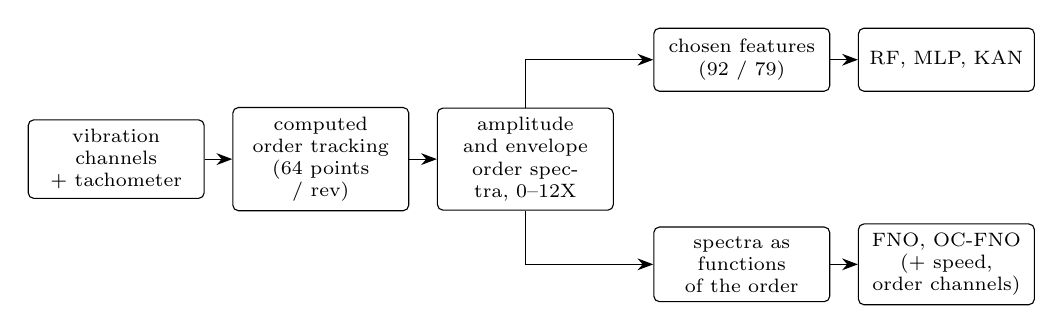
\begin{tikzpicture}[node distance=3mm and 3.5mm, every node/.style={font=\scriptsize, align=center},
  box/.style={draw, rounded corners=2pt, minimum height=8mm, text width=20mm}, >={Stealth[length=2mm]}]
\node[box] (raw) {vibration channels\\+ tachometer};
\node[box, right=of raw] (ord) {computed order tracking\\(64 points / rev)};
\node[box, right=of ord] (spec) {amplitude and envelope\\order spectra, 0--12X};
\node[box, above right=2mm and 5mm of spec] (feat) {chosen features\\(92 / 79)};
\node[box, below right=2mm and 5mm of spec] (op) {spectra as functions\\of the order};
\node[box, right=of feat] (m1) {RF, MLP, KAN};
\node[box, right=of op] (m2) {FNO, OC-FNO\\(+ speed, order channels)};
\draw[->] (raw) -- (ord); \draw[->] (ord) -- (spec); \draw[->] (spec) |- (feat); \draw[->] (spec) |- (op);
\draw[->] (feat) -- (m1); \draw[->] (op) -- (m2);
\end{tikzpicture}
\caption{Processing chain shared by every model. The Hamiltonian-energy baseline uses decimated waveforms of the
bearing accelerometers instead of the spectra (Section~\ref{sec:models}).}
\label{fig:pipeline}
\end{figure}

\subsection{Models}
\label{sec:models}

\paragraph{Feature models} A random forest \citep{breiman2001rf} (500 trees, class-balanced), an MLP (two hidden
layers of 128 and 64 units, L2 penalty $10^{-3}$) and a shallow KAN \citep{liu2024kan} (one hidden layer of 16
units; every edge $\phi(x)=w\,\mathrm{silu}(x)+\sum_k c_k B_k(x)$ with cubic B-splines on eight intervals),
following the shallow design of Rigas et al.~\citep{rigas2024kan} without their feature selection.

\paragraph{Hamiltonian-energy baseline} In the spirit of Shen et al.~\citep{shen2023hnn}, a Hamiltonian neural network
\citep{greydanus2019hnn} with one degree of freedom learns $H(q,p)$ from the orbits of the bearing housings
($q$ the radial and $p$ the tangential acceleration, standardised per run, time in shaft revolutions), on the healthy
runs of the training split only. The features of a run are the mean and the coefficient of variation of the learned
energy, the mean energy rate $|\nabla H\cdot\dot z|$ and the residual of Hamilton's equations, for both bearings; a
random forest classifies them.

\paragraph{FNO} The spectra (14 or 12 channels, 0--8 orders) are log-scaled and lifted to 32 channels; three spectral
blocks ($x\leftarrow\mathrm{GELU}(\mathcal{K}x+Wx)$, 48 Fourier modes) are followed by mean and max pooling over the
order axis, the speed is appended and a small MLP gives the class \citep{li2021fno}.

\paragraph{Order-conditioned FNO (OC-FNO)} Four changes, each with a physical reason: (i) per-channel normalisation
estimated on the training split only, AdamW with a one-cycle learning rate ($10^{-3}$), gradient clipping, dropout and
label smoothing; (ii) FiLM conditioning \citep{perez2018film} of every spectral block on the speed,
$h\leftarrow h\odot(1+\gamma(v))+\beta(v)$, because the line amplitudes depend on speed through the structure's
transfer function; (iii) two input channels that mark the physical orders, Gaussian combs at the harmonics $k$X and at
the bearing orders; (iv) a transfer-function augmentation, a random log-normal gain ($\sigma=0.3$) per sensor applied
to its amplitude and envelope spectra, because the order of a line does not move with speed but its amplitude does.

\subsection{Protocols and metrics}

Every run is one sample, so no part of a recording is ever on both sides of a split. \textbf{Pa}: stratified 5-fold
cross-validation by run (test speeds interleaved with training speeds). \textbf{Pb}: the runs are divided into speed
terciles; a model is trained on two terciles and tested on the third, in turn (the low and high terciles are
extrapolation in speed). Tasks: T1 misalignment (normal / horizontal / vertical, 547 runs), T2 unbalance (normal /
imbalance, 382), T3 bearings (normal / six bearing faults, 1064), T4 all ten MAFAULDA states (1895) and C1 the seven
COMFAULDA states (2161). The metric is the macro-F1 pooled over the test folds; seeds change the folds and the
initialisation (5 seeds for the random forest, MLP, KAN and OC-FNO, 3 for the FNO, 1 for the Hamiltonian baseline and
the ablations), and intervals are 95\,\% $t$-intervals over seeds. For compound faults, one binary detector per fault
type (unbalance, horizontal, vertical) is trained on the normal and single-fault COMFAULDA runs and applied to the
combined runs; the exact match requires the three labels to be right.

%% -------------------------------------------------------------------------------------------------------------
\section{Results}
\label{sec:results}

\subsection{Seen speeds}

When the test speeds are interleaved with the training speeds (Table~\ref{tab:seen}), the feature models reach
0.985--0.994 on every MAFAULDA task and 0.938--0.944 on COMFAULDA, the level reported in the literature
\citep{rigas2024kan}; the FNO is slightly lower and more variable between seeds, and the Hamiltonian-energy baseline
stays at 0.76--0.93, consistent with Shen et al.~\citep{shen2023hnn}.

\begin{table*}[t]
\centering
\caption{Macro-F1 when the test speeds are seen in training (Pa: stratified 5-fold by run). Mean $\pm$ 95\% interval over seeds (RF, MLP, KAN: 5; FNO: 3 on MAFAULDA); single values: one seed.}
\label{tab:seen}
\resizebox{\textwidth}{!}{%
\begin{tabular}{lccccc}
\toprule
Task & RF & MLP & KAN & FNO & HNN+RF \\
\midrule
T1 misalignment & 0.988\,$\pm$\,0.003 & 0.985\,$\pm$\,0.003 & 0.986\,$\pm$\,0.003 & 0.970\,$\pm$\,0.058 & 0.758 \\
T2 unbalance & 0.990\,$\pm$\,0.006 & 0.991\,$\pm$\,0.006 & 0.991\,$\pm$\,0.006 & 0.990\,$\pm$\,0.022 & 0.932 \\
T3 bearings & 0.994\,$\pm$\,0.001 & 0.988\,$\pm$\,0.004 & 0.992\,$\pm$\,0.001 & 0.987\,$\pm$\,0.005 & 0.821 \\
T4 all ten states & 0.992\,$\pm$\,0.001 & 0.986\,$\pm$\,0.001 & 0.989\,$\pm$\,0.002 & 0.975\,$\pm$\,0.015 & 0.760 \\
C1 COMFAULDA & 0.944 & 0.938 & 0.938 & 0.913 & -- \\
\bottomrule
\end{tabular}}
\end{table*}


\subsection{Unseen speeds}

Holding out a speed tercile changes the picture (Table~\ref{tab:unseen}, Fig.~\ref{fig:protocols}). Every model loses
0.11--0.18 macro-F1 on MAFAULDA and 0.25--0.32 on COMFAULDA. The random forest is the most accurate model on T1, T3 and
T4 and by far the most stable (standard deviation over seeds at most 0.008); the plain FNO is below it on every task
and its seed-to-seed spread is three to ten times larger. The MLP is best on COMFAULDA (0.690). Errors concentrate in
the outer terciles (Fig.~\ref{fig:bands}): the middle tercile, which is interpolation, stays close to 1.0, whereas the
low tercile (12--27\,Hz) is the hardest on every task.

\begin{table*}[t]
\centering
\caption{Macro-F1 at unseen rotation speeds (Pb: each speed tercile held out in turn). Mean $\pm$ 95\% interval over seeds; single values: one seed.}
\label{tab:unseen}
\resizebox{\textwidth}{!}{%
\begin{tabular}{lcccccc}
\toprule
Task & RF & MLP & KAN & FNO & HNN+RF & OC-FNO \\
\midrule
T1 misalignment & 0.876\,$\pm$\,0.009 & 0.838\,$\pm$\,0.029 & 0.858\,$\pm$\,0.016 & 0.800\,$\pm$\,0.137 & 0.629 & 0.763\,$\pm$\,0.028 \\
T2 unbalance & 0.852\,$\pm$\,0.010 & 0.884\,$\pm$\,0.015 & 0.873\,$\pm$\,0.009 & 0.864\,$\pm$\,0.187 & 0.759 & 0.933\,$\pm$\,0.022 \\
T3 bearings & 0.866\,$\pm$\,0.010 & 0.837\,$\pm$\,0.004 & 0.811\,$\pm$\,0.011 & 0.803\,$\pm$\,0.059 & 0.541 & 0.816\,$\pm$\,0.026 \\
T4 all ten states & 0.878\,$\pm$\,0.003 & 0.817\,$\pm$\,0.006 & 0.824\,$\pm$\,0.017 & 0.800\,$\pm$\,0.043 & 0.508 & 0.763\,$\pm$\,0.058 \\
C1 COMFAULDA & 0.634\,$\pm$\,0.008 & 0.690\,$\pm$\,0.010 & 0.641\,$\pm$\,0.020 & 0.690 & -- & 0.589\,$\pm$\,0.029 \\
\bottomrule
\end{tabular}}
\end{table*}


\begin{figure}[t]
\centering
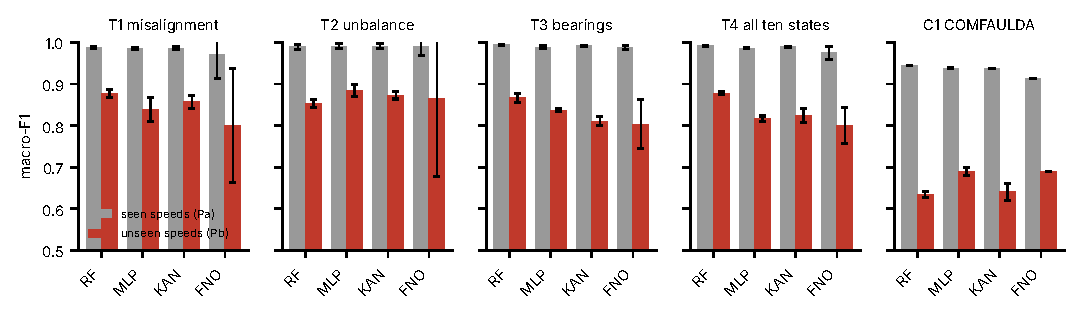
\includegraphics[width=\textwidth]{figures/fig_protocols.pdf}
\caption{Macro-F1 with the test speeds seen in training (Pa, grey) and held out (Pb, red); bars: mean over seeds,
whiskers: 95\,\% interval.}
\label{fig:protocols}
\end{figure}

\subsection{Order-conditioned FNO}

The OC-FNO generalises clearly better than every other model for unbalance (Table~\ref{tab:gain}): 0.933 against 0.852
for the random forest, a difference that is positive for each of the five seeds, and up to 1.00 in the high tercile,
where the random forest falls to 0.66 (Fig.~\ref{fig:bands}). It is below the random forest on the four other tasks,
by 0.04--0.12. The ablation (Table~\ref{tab:ablation}) locates the cause: removing the FiLM speed conditioning raises
T4 from 0.721 to 0.827 and C1 from 0.594 to 0.699, while removing the order channels or the gain augmentation changes
little. The OC-FNO also reduces the seed-to-seed spread of the FNO on unbalance (standard deviation 0.018 against
0.075).

\begin{table}[t]
\centering
\caption{Order-conditioned FNO against the random forest at unseen speeds (Pb): macro-F1 (mean $\pm$ 95\% interval over seeds) and the paired same-seed difference.}
\label{tab:gain}
\resizebox{\columnwidth}{!}{%
\begin{tabular}{lcccc}
\toprule
Task & OC-FNO & RF & OC-FNO $-$ RF & Seeds $>0$ \\
\midrule
T1 misalignment & 0.763\,$\pm$\,0.028 & 0.876\,$\pm$\,0.009 & $-0.114\pm0.020$ & 0/5 \\
T2 unbalance & 0.933\,$\pm$\,0.022 & 0.852\,$\pm$\,0.010 & $+0.081\pm0.027$ & 5/5 \\
T3 bearings & 0.816\,$\pm$\,0.026 & 0.866\,$\pm$\,0.010 & $-0.051\pm0.022$ & 0/5 \\
T4 all ten states & 0.763\,$\pm$\,0.058 & 0.878\,$\pm$\,0.003 & $-0.115\pm0.060$ & 0/5 \\
C1 COMFAULDA & 0.589\,$\pm$\,0.029 & 0.634\,$\pm$\,0.008 & $-0.043\pm0.035$ & 0/4 \\
\bottomrule
\end{tabular}}
\end{table}

\begin{table}[t]
\centering
\caption{Ablation of the order-conditioned FNO at unseen speeds (macro-F1, seed 0; -- not run).}
\label{tab:ablation}
\footnotesize
\begin{tabular}{lcc}
\toprule
Variant & T4 MAFAULDA & C1 COMFAULDA \\
\midrule
Full OC-FNO & 0.721 & 0.594 \\
without FiLM speed conditioning & 0.827 & 0.699 \\
without order channels & 0.749 & -- \\
without gain augmentation & 0.739 & 0.591 \\
\bottomrule
\end{tabular}
\end{table}


\begin{figure}[t]
\centering
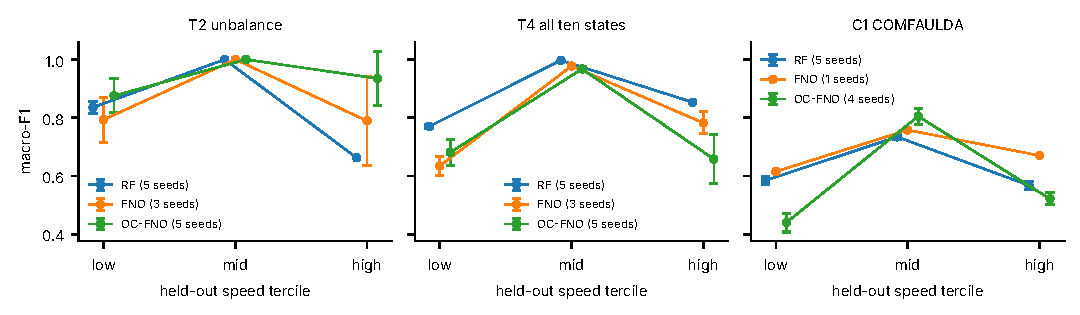
\includegraphics[width=\textwidth]{figures/fig_speed_bands.pdf}
\caption{Macro-F1 of the held-out speed tercile for the random forest, the FNO and the OC-FNO (mean and standard
deviation over seeds).}
\label{fig:bands}
\end{figure}

\subsection{Compound faults from single-fault training}

Trained on normal and single-fault runs, the detectors do not recognise compound faults (Table~\ref{tab:composition}):
the exact pair is right in 1.5--5.2\,\% of the 1143 combined runs. Unbalance is still detected inside the combinations
(F1 0.76--0.86), misalignment is not (0.38--0.53).

\begin{table}[t]
\centering
\caption{Combined faults recognised from single-fault training on COMFAULDA: one detector per fault type trained on 1018 normal and single-fault runs, tested on 1143 combined-fault runs never seen. Exact match: all three labels right.}
\label{tab:composition}
\resizebox{\columnwidth}{!}{%
\begin{tabular}{lcccc}
\toprule
Model & Exact match & F1 unbalance & F1 horizontal & F1 vertical \\
\midrule
RF & 0.015 & 0.86 & 0.38 & 0.42 \\
MLP & 0.052 & 0.81 & 0.45 & 0.53 \\
KAN & 0.050 & 0.76 & 0.45 & 0.47 \\
\bottomrule
\end{tabular}}
\end{table}


\subsection{Recording-session artefacts in MAFAULDA}

Three properties of the recordings matter for any method that uses phase or channel-level information. (i) Spurious
or missing tachometer pulses affect 56 runs, concentrated in the underhang ball-fault folder. (ii) The 1X phase,
referred to the tachometer pulse, is not consistent between mass levels: with one free complex unbalance per level,
its magnitude follows the added mass (6.6 to 35\,g for 6 to 35\,g) but its angle drifts from 44 to 0\,deg across the
imbalance sessions (Fig.~\ref{fig:level}), and spans 20--38\,deg inside each of the six bearing-fault folders. (iii)
In some sessions the overhang radial accelerometer reads up to 66 times its healthy 1X amplitude; a channel-screened
estimate of the unbalance mass (Tukey biweight of the per-channel estimates) rejects it in 99\,\% of the affected runs
and divides the cross-session error of the mass estimate by five, from 19.4 to 3.79\,g.

\begin{figure}[t]
\centering
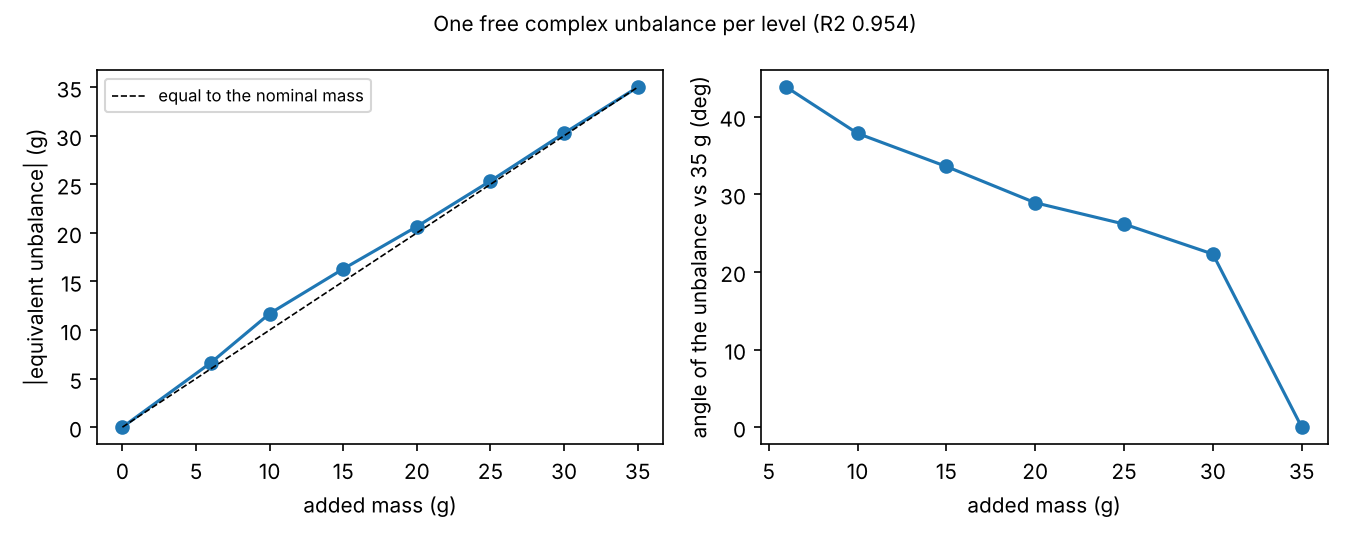
\includegraphics[width=0.85\textwidth]{figures/fig_level_unbalance.png}
\caption{One free complex unbalance per mass level fitted to the 1X phasors of the six MAFAULDA accelerometers:
magnitude against the added mass (left) and angle relative to the 35\,g level (right).}
\label{fig:level}
\end{figure}

%% -------------------------------------------------------------------------------------------------------------
\section{Discussion}
\label{sec:discussion}

\paragraph{Why speed generalisation fails} After order tracking, the positions of the fault lines no longer depend on
speed; their amplitudes still do, through the transfer function of the bench and its resonances. Modal fits of the
MAFAULDA 1X response place resonances around 9 and 19\,Hz, inside or next to the low tercile, which is the hardest for
every model. A model trained on the middle and high speeds therefore sees, at low speed, signatures of the right
orders but of amplitudes it has never met. Interleaved splits hide this because every test speed has neighbours in
training; the drop of 0.11--0.32 measured here is the cost of that hidden interpolation.

\paragraph{When conditioning on speed helps} The unbalance signature is a single order (1X) whose amplitude grows
smoothly with speed: conditioning the operator on speed lets it learn that dependence and extrapolate it, which is
why the OC-FNO reaches 0.933. For misalignment and bearing faults, the discriminative information lies in ratios
between orders, directions and envelope lines; speed-dependent modulation fitted on two terciles then extrapolates
badly to the third, and removing it brings the OC-FNO close to the random forest. Speed conditioning should therefore
be restricted to the signatures whose speed dependence is physically simple, or replaced by a physical model of the
transfer function.

\paragraph{Compound faults} The failure of composition shows that, with these phase-free order features, the
signature of a combined fault is not the union of the single ones: misalignment changes how the rotor responds to
unbalance and vice versa. Recognising compound faults will require training data that contain them or a mechanical
model of their interaction.

\paragraph{Limitations} The study uses one bench type, records of five seconds (which cannot separate the outer- and
inner-race orders from 3X and 5X), labels taken from the database folders, and a re-implementation of the KAN and
Hamiltonian baselines rather than the authors' code. The Hamiltonian baseline and the ablations were run with one seed
because of their cost. The FNO hyper-parameters were not tuned beyond the changes stated; a larger search might narrow
the gap, but it would have to be made under the same speed-held-out protocol.

%% -------------------------------------------------------------------------------------------------------------
\section{Conclusions}
\label{sec:conclusions}

Under a protocol that holds out whole speed terciles and never splits a recording, fault classifiers that score above
0.97 on MAFAULDA and COMFAULDA lose 0.11--0.32 macro-F1. A random forest on order-domain features is the most accurate
and stable model overall; an order-conditioned Fourier neural operator is the best model for unbalance, and its speed
conditioning, which helps unbalance, hurts the faults whose signatures are ratios between orders. Compound faults are
not recognised from single-fault training. Reporting speed-held-out results, with seed-level intervals, should become
standard on these databases.

%% -------------------------------------------------------------------------------------------------------------
\section*{CRediT authorship contribution statement}
\textbf{First Author:} Conceptualization, Methodology, Software, Investigation, Writing -- original draft.
\textbf{Second Author:} Supervision, Writing -- review \& editing. (To be completed by the authors.)

\section*{Declaration of competing interest}
The authors declare that they have no known competing financial interests or personal relationships that could have
appeared to influence the work reported in this paper.

\section*{Declaration of generative AI and AI-assisted technologies in the writing process}
During the preparation of this work the authors used an AI assistant (Claude, Anthropic) to write analysis code and to
draft the manuscript. After using this tool, the authors reviewed and edited the content as needed and take full
responsibility for the content of the publication.

\section*{Data availability}
MAFAULDA and COMFAULDA are publicly available \citep{mafaulda,comfaulda}. The code, the extracted-feature pipeline, the
protocols written before each experiment and every result file are available at \citep{pinneapple}.

\section*{Funding}
To be completed by the authors.

\bibliographystyle{elsarticle-num}
\bibliography{references}

\end{document}
